\section{Experimental Study}
\label{sec:exp}
In this section, we evaluate the efficiency and scalability of our proposed distributed GCMP detectors on real trajectory datasets. All the experiments are carried out in a cluster with $12$ nodes, each equipped with four quad-core $2.2$GHz Intel processors, $32$GB memory and gigabit Ethernet. 
%The cluster is installed with CentOS 5.5. operating system.

\textbf{Environment Setup}: We use Yarn\footnote{http://hadoop.apache.org/docs/current/hadoop-yarn/hadoop-yarn-site/YARN.html} to manage our cluster. We pick one machine as the Yarn's master node, and the remainings reserve one core and $2$GB memory for Yarn processes. We deployed our GCMP detector on Apache Spark 1.5.5~\cite{zaharia2012resilient} with the remaining $11$ nodes as the computing nodes.
To fully utilize the computing resources, we configure each node to run five executors, each taking three cores and $5$GB memory. In Spark, one of the $55$ executor is taken as the Application Master for coordination, therefore our setting results in $54$ executors.
All our implementations as well as cluster setups are open-sourced in XXX.
%can be referred in our 
%We use ``yarn-cluster'' mode
%for Spark which randomly picks one executor to act as the Application Master. Such a configuration allows us to run 162 tasks
%at the same time. We use HDFS as our storage engine with replicator factor of 1.
%The summary of the configuration is as in the following table:

\eat{
\begin{table} [h]
\centering
\begin{tabular}{|l|c|}
\hline 
Parameter & Value  \\ 
\hline 
Java Version & 1.7.0 \\ 
\hline 
Spark Version & 1.5.5 \\ 
\hline 
spark.driver.memory & 2GB \\ 
\hline 
spark.executor.cores & 3  \\ 
\hline 
spark.executor.instances & 54 \\ 
\hline 
spark.executor.memory & 5GB \\ 
\hline 
spark.master & yarn-cluster \\
\hline 
spark.serializer & KryoSerializer \\ 
\hline 
\end{tabular} 
\end{table}
}


\textbf{Datasets}: We use three real trajectory datasets in different application scenarios:
\begin{itemize}
\item{Geolife}~\footnote{http://research.microsoft.com/en-us/projects/geolife/}. The dataset essentially keeps all the travel records of 182 users for a period
of over three years, including multiple kinds of transportation modes (walking, driving and taking public
transportation). For each user, the GPS information is collected periodically and 91 percent of the trajectories
are sampled every 1 to 5 seconds.
\item{Shopping}\footnote{http://www.irc.atr.jp/crest2010\_HRI/ATC\_dataset/}. The dataset contains
  trajectories of visitors in the ATC shopping center in Osaka. To better capture the indoor activities, the visitor locations are sampled every half second, resulting in $13,183$ long trajectories. 
\item{Taxi}. The dataset tracks the trajectories of $15,054$ taxies in Singapore over August 2008. The sampling
rate is around 30 seconds. 
\end{itemize}


\textbf{Preprocessing}: We replace timestamps with global sequences (starting from $1$) for each dataset. 
We set a fixed sampling rate for each dataset (i.e., Geolife = 5 seconds, Shopping=0.5 seconds, Taxi = 30 seconds)
and use linear interpolation to fill missing values.
%For each dataset, we set a fixed sampling rate (CLEARLY STATE THE SAMPLING RATE FOR EACH DATASET) and use linear interpolation to fill missing values. 
%Finally, we obtain a set of trajectories with equal length. 
%Finally, we obtain a set of dense trajectories with equal length. 
For the clustering method, we use DBSCAN~\cite{ester1996density} and customize its two parameters $\epsilon$ and $minPt$~\footnote{$\epsilon$ is the maximum neighborhood range to be concerned, $minPt$ is the minimum number of objects to form a dense region.}. We set $\epsilon=5$, $minPt=10$ for GeoLife and Shopping datasets; and $\epsilon=20$, $minPt=10$ for Taxi dataset. Note that other clustering methods and settings can also be applied. The clustered snapshots are stored in HDFS as $\langle t, S_t \rangle$ pair, where $t$ is the timestamp, $S_t$ contains the clusters at snapshot $t$. 
After preprocessing, the statistics of the three datasets are presented in Table~\ref{exp:dataset}. 

\begin{table} [h]
\center
\small
\begin{tabular}{|l|l|l|l|}
\hline
 \textbf{Attributes}& \textbf{Shopping} &  \textbf{Geolife} &  \textbf{SingTaxi} \\ 
\hline 
\# objects  & 13,183 & 18,670 & 15,054\\ 
\hline
%\# average ts & 3,114  & 2,924 & 19,667 \\ 
%\hline
\# data points  & 41,052,242 & 54,594,696 & 296,075,837\\ 
\hline
\# snapshots  & 16,931 & 10,699 & 44,364\\ 
\hline
\# clusters  & 211,403  & 206,704& 536,804\\
\hline
avg. cluster size  & 171 & 223 & 484\\
\hline
%\# of patterns & 3,741 & 4,369  & 7,585 \\
%\hline
\end{tabular}
\caption{Statistics of data set}
\label{exp:dataset}
\end{table}

\textbf{Parameters}: To systematically study the performance of
our algorithms, we conduct experiments on various parameter settings. The parameters to be evaluated are listed in Table~\ref{tbl:parameters}, with default settings in bold. 
\begin{table}[h]
\small
\begin{tabular}{c|l|l}
\hline 
\textbf{Variables} & \textbf{Meaning} & \textbf{Values} \\ 
\hline 
M & min size of object set &  5, 10,  \textbf{15}, 20, 25 \\ 
\hline 
K & min duration & 120, 150, \textbf{180}, 210, 240 \\ 
\hline 
L & min local duration & 10, 20, \textbf{30}, 40,50 \\ 
\hline 
G & max gap & 10, 15, \textbf{20}, 25, 30 \\ 
\hline
$O_r$ & ratio of objects & 20\%,40\%, 60\%, 80\%, \textbf{100\%} \\ \hline
$T_r$ & ratio of snapshots & 20\%,40\%, 60\%, 80\%, \textbf{100\%} \\ \hline
N & number of machines & 1, 3, 5, 7, 9, \textbf{11}\\ 
\hline 
\end{tabular} 
\caption{Variables and their default values}
\label{tbl:parameters}
\end{table}




\eat{
\textbf{Number of patterns under different parameters}: We first 
analyze the number of patterns exist in each dataset under different conditions. The results are presented in Figures~\ref{exp:patterns_vary}. As expected, the number of patterns differs under in different scenarios. Larger $M$, $L$, $K$ imply smaller number of patterns, because lesser patterns are able to meet stricter $M$, $L$, $K$ constraints. In contrast, larger $G$ implies larger number of patterns. This is because larger gaps relaxes the pattern constraint. Two interesting observations are made on $L$ and $G$.
First, as $L$ increases from $10$ to $20$, the number of patterns drops quickly (50\% less). Second, opposed to $L$'s trend, as $G$ reaches to $30$ from $25$, the number of patterns bursts (near 50\% more). The distribution of patterns under $G$ and $L$ reveals that there are many companions in real life which are short and intermittent. With GCMP, we can discover these patterns by properly adjusting $L$ and $G$s.


\begin{figure}[h]
\centering
 	 \begin{subfigure}[b]{0.23\textwidth}
        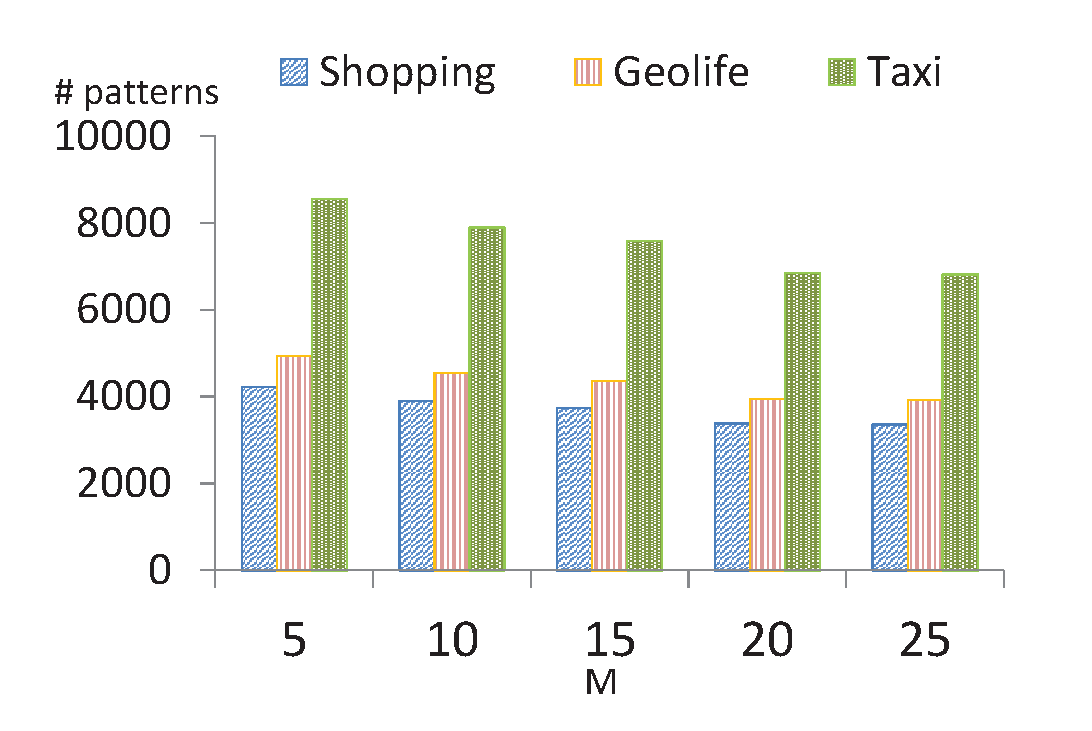
\includegraphics[width=\textwidth]{/exp/effectiveness/patterns_vary_M.eps}
        \caption{Number of patterns vary $M$}
    \end{subfigure}
    \begin{subfigure}[b]{0.23\textwidth}
        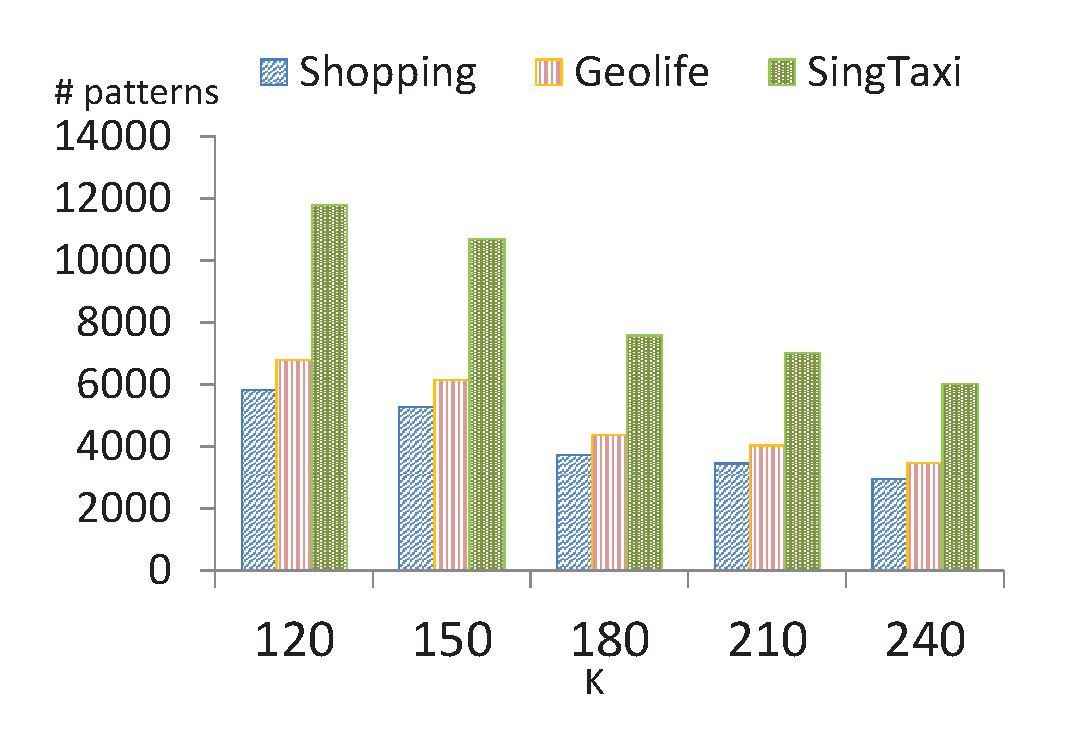
\includegraphics[width=\textwidth]{/exp/effectiveness/patterns_vary_K.eps}
        \caption{Number of patterns vary $K$}
    \end{subfigure}  
    \begin{subfigure}[b]{0.23\textwidth}
        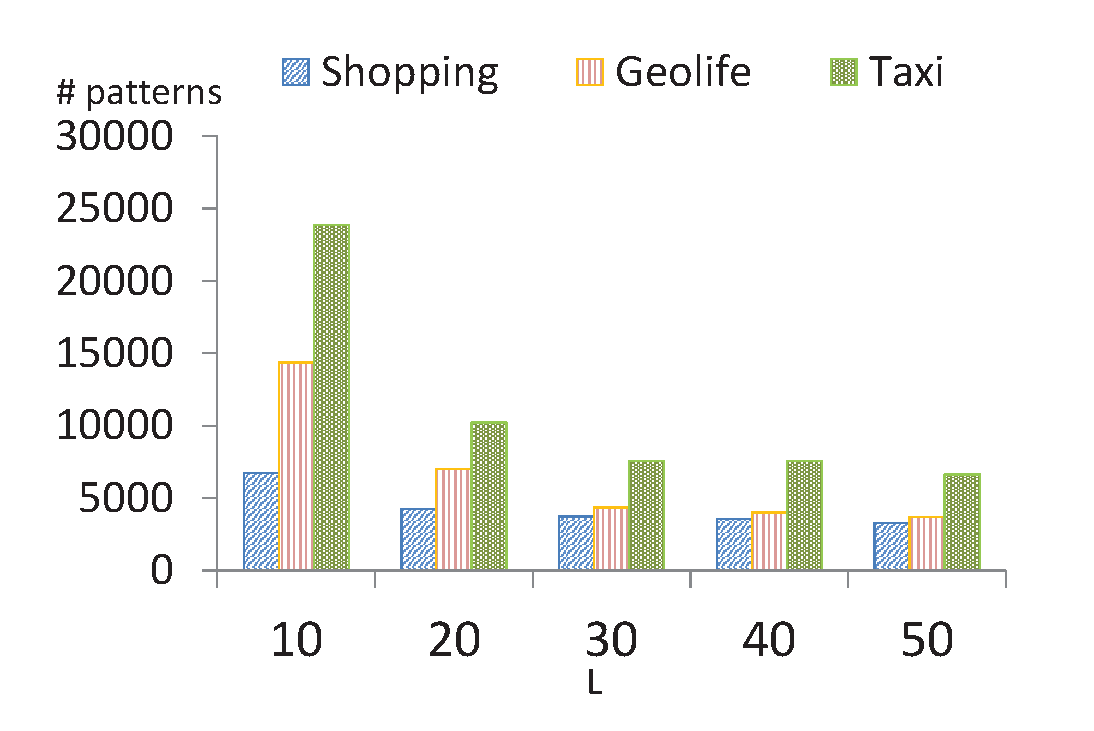
\includegraphics[width=\textwidth]{/exp/effectiveness/patterns_vary_L.eps}
        \caption{Number of patterns vary $L$}
    \end{subfigure}
    \begin{subfigure}[b]{0.23\textwidth}
        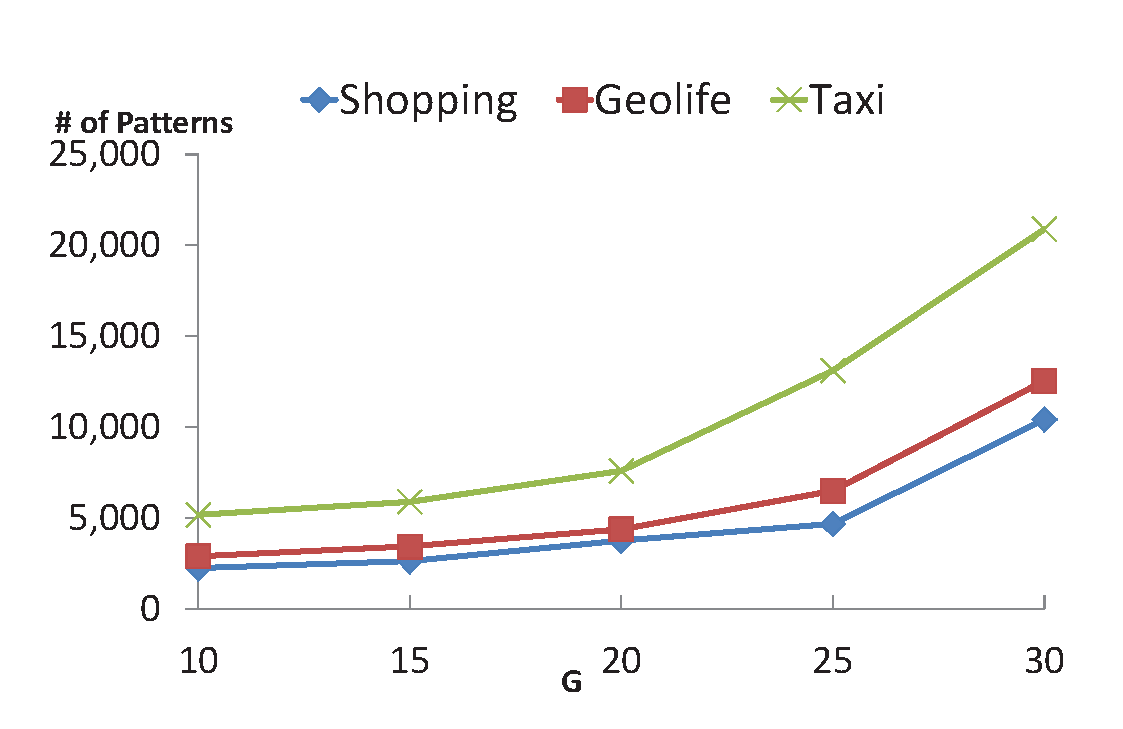
\includegraphics[width=\textwidth]{/exp/effectiveness/patterns_vary_G.eps}
        \caption{Number of patterns vary $G$}
    \end{subfigure}    
\caption{Number of patterns discovered from real datasets}
\label{exp:patterns_vary}
\end{figure}
}

\eat{
\textbf{Algorithms}: We implement TRPM, SPARE and SPARE-LB for comparison study. TRPM and SPARE are implement as described in Section 4 and 5. SPARE-LB extends SPARE by appending an additional load balance stage to the map phase. 
When the mappers complete, SPARE-LB collects the size of stars from all mappers. 
Then a best-fit strategy is applied for task allocation. In best-fit, 
tasks are assigned in decreasing order of their sizes, and the most costly
unassigned task is allocated to the current mostly empty reducer. 
In SPARE-LB, we simply use the number of edges in stars as a cost estimation. The remaining
parts of SPARE-LB are identical to SPARE.
}



\subsection{Performance Evaluation}
\eat{
Since the both TRPM and SPARE utilizes pruning rules that related to the pattern parameters $M$,$K$,$L$,$G$. It is interesting to
see their performances under different settings.
We run the three algorithms using all three datasets 
and report their overall performances in Figures~\ref{exp:performance_vary}.
In brief, all of the three algorithms 
are able to handle the large-scaled real
datasets. However, SPARE algorithms are obviously more efficient than TRPM. 
In the case when $G$ is large (i.e., $G=30$), 
TRMP takes near three hours for Taxi dataset, which is 15 times slower than SPARE algorithms. Besides, SPARE-LB is consistently more efficient than SPARE, with an average of 20\% improvements.
Another general observation
is that all of the three algorithms run slower in the Taxi dataset as compared to
other two datasets. This is because Taxi dataset contains
the most number of temporal data points, which is around 7 times of Shopping
dataset and 5 times of geolife dataset.
 In summary, SPARE outperforms TRMP in all cases. Next, we analyze the details of each experiments.
}
\begin{figure*}[t]
\centering
    \begin{subfigure}[b]{0.23\textwidth}
        \includegraphics[width=\textwidth]{/exp/performance/shopping_vary_M.eps}
        \caption{Shopping vary $M$}
    \end{subfigure}
    \begin{subfigure}[b]{0.23\textwidth}
        \includegraphics[width=\textwidth]{/exp/performance/shopping_vary_K.eps}
        \caption{Shopping vary $K$}
    \end{subfigure}
    \begin{subfigure}[b]{0.23\textwidth}
        \includegraphics[width=\textwidth]{/exp/performance/shopping_vary_L.eps}
        \caption{Shopping vary $L$}
    \end{subfigure}
       \begin{subfigure}[b]{0.23\textwidth}
        \includegraphics[width=\textwidth]{/exp/performance/shopping_vary_G.eps}
        \caption{Shopping vary $G$}
    \end{subfigure}

	\begin{subfigure}[b]{0.23\textwidth}
        \includegraphics[width=\textwidth]{/exp/performance/geolife_vary_M.eps}
        \caption{Geolife vary $M$}
    \end{subfigure}
    \begin{subfigure}[b]{0.23\textwidth}
        \includegraphics[width=\textwidth]{/exp/performance/geolife_vary_K.eps}
        \caption{Geolife vary $K$}
    \end{subfigure}
    \begin{subfigure}[b]{0.23\textwidth}
        \includegraphics[width=\textwidth]{/exp/performance/geolife_vary_L.eps}
        \caption{Geolife vary $L$}
    \end{subfigure}
       \begin{subfigure}[b]{0.23\textwidth}
        \includegraphics[width=\textwidth]{/exp/performance/geolife_vary_G.eps}
        \caption{Geolife vary $G$}
    \end{subfigure}
    
    \begin{subfigure}[b]{0.23\textwidth}
        \includegraphics[width=\textwidth]{/exp/performance/taxi_vary_M.eps}
        \caption{Taxi vary $M$}
    \end{subfigure}
    \begin{subfigure}[b]{0.23\textwidth}
        \includegraphics[width=\textwidth]{/exp/performance/taxi_vary_K.eps}
        \caption{Taxi vary $K$}
    \end{subfigure}
    \begin{subfigure}[b]{0.23\textwidth}
        \includegraphics[width=\textwidth]{/exp/performance/taxi_vary_L.eps}
        \caption{Taxi vary $L$}
    \end{subfigure}
       \begin{subfigure}[b]{0.23\textwidth}
        \includegraphics[width=\textwidth]{/exp/performance/taxi_vary_G.eps}
        \caption{Taxi vary $G$}
    \end{subfigure}       
\caption{Performance of SPARE and TRPM on real datasets under different pattern parameters.}
\label{exp:performance_vary}
\end{figure*}
%\subsubsection{Effects of pattern parameters M,L,K,G}
\textbf{Varying $M$}: Figures~\ref{exp:performance_vary} (a),(e),(i)
present the performance with increasing $M$. The SPARE framework demonstrates a clear superiority over TRPM framework, with a boosting factor of  $2.7$ times in Shopping, $3.1$ times in Geolife and
$7$ times in Taxi. As $M$ increases, the running time of both frameworks slightly improves because the number of clusters in each snapshot drops, generating fewer valid candidates.


\textbf{Varying $K$}: The performance with increasing $K$ is shown in Figure~\ref{exp:performance_vary} (b),(f),(j).  SPARE tends to run faster, whereas the performance of TRPM degrades dramatically. This is caused by the \emph{sequence simplification} procedure in SPARE, which can prune many candidates with large $K$. However, the line sweep algorithm in TRPM does not utilize such property for pruning. It takes longer time because more replication data has to be handled in each partition.



%Second, when $K$ is very small (i.e, $K=0.XXX|T|$), TRPM could outperform SPARE because smaller $K$ indicates small partition size in TRPM but restricted the pruning power in SPARE. As a result, TRPM wins 10\% in Geolife dataset. However, by leveraging the load balancing, SPARE-LB is still faster than TRPM.

\textbf{Varying $L$}: Figures~\ref{exp:performance_vary} (c)(g)(k) present the performances with varying $L$. When $L=10$, SPARE can outperform TRPM by around $10$ times. We also observe that there is a significant performance improvement for TPRM when $L$ increases from $10$ to $20$ and later the running time drops smoothly. 
This is because $\eta$ is proportional to $O(L + 1/L)$. When $L$ is small (i.e., from $10$ to $20$),
$\eta$ decreases quickly (i.e., 30\%). As $L$ further increases (e.g, from $20$ to $30$),
$\eta$ decreases steadily (e.g, 15\%).
%CAN YOU EXPLAIN THIS FROM THE RELATIONSHIP between $\eta$ and $L$. 

\eat{
An interesting observation is that $L$
provides good pruning power from $10$ to $20$ for both TRPM and SPARE based algorithms. The major reason is that the decrease of $L$ invalidates many candidates (as shown in Figure~\ref{exp:patterns_vary} (c)), thus the prunings in both SPARE and TRPM become more significant. 

 As $L$ continues to increase, we can see that TRPM's performance gain is larger than SPARE based algorithms. This is because larger $L$ indicates smaller $\eta$, which is more beneficial to TRPM.
}


\textbf{Varying $G$}: Figures~\ref{exp:performance_vary} (d)(h)(l) present the performances with increasing $G$.  TRPM is rather sensitive to $G$. When $G$ is relaxed to larger values, more valid patterns would generate. TPRM has to set a higher replication factor and its running time degrades drastically when $G$ increases from $20$ to $30$. In contrast, with much more effective pruning strategy, our SPARE scales very well with $G$.

\eat{
We can see that both TRPM and SPARE run slower. The reason is that large $G$ relaxes the constraint of a pattern, thus the pruning powers of TRPM and SPARE is more restricted. We observe that there is a burst in performance of TRPM when $G$ reach to $30$. The major reason is that when $G$ becomes to 30, the number of valid patterns almost doubles as shown in Figure~\ref{exp:patterns_vary} (d). This indicate that during TRPM's line sweep, very few patterns can be pruned, making the candidate set grows exponentially. Similarly, SPARE algorithms are also affected by the increase of $G$. However we do not observe such a burst for SPARE. The reason is bi-folded. First, SPARE can utilize $K$, $L$ to retain the power of pruning. Second, SPARE leverages \emph{forward closure check} to quickly output valid patterns and avoids to enumerating many candidates.
}
\textbf{Varying $O_r$}: Figures~\ref{exp:performance_vary_OT} (a)(b)(c) present 
the performances wrt. increasing number of total objects. The x-axis are the ratio
of objects sampled from the corresponding datasets. We can see that the performance of
both TRPM and SPARE decreases linearly to the the number of total objects. This
is reasonable since larger $O_r$ results in more clusters per snapshot, which affects
the line-sweep in TRPM and the aggregate graph in SPARE. However in all cases, SPARE
consistently outperforms TRPM.

\textbf{Varying $T_r$}: Figures~\ref{exp:performance_vary_OT} (d)(e)(f) present 
the performances wrt. increasing number of total snapshots.  The x-axis represents the size of
snapshots sampled from the corresponding datasets. We again observe the linear decrease of
the performances wrt. the number of snapshots. In all cases, SPARE is faster than
TRPM. We further observe that as $T_r$ grows, the gaps between SPARE and TRPM tends
to be larger, this is because larger $T_r$ results larger partition size, and more 
snapshots needs to be swept in TRPM.

\begin{figure}[h]
\centering
	\begin{subfigure}[b]{0.22\textwidth}
	 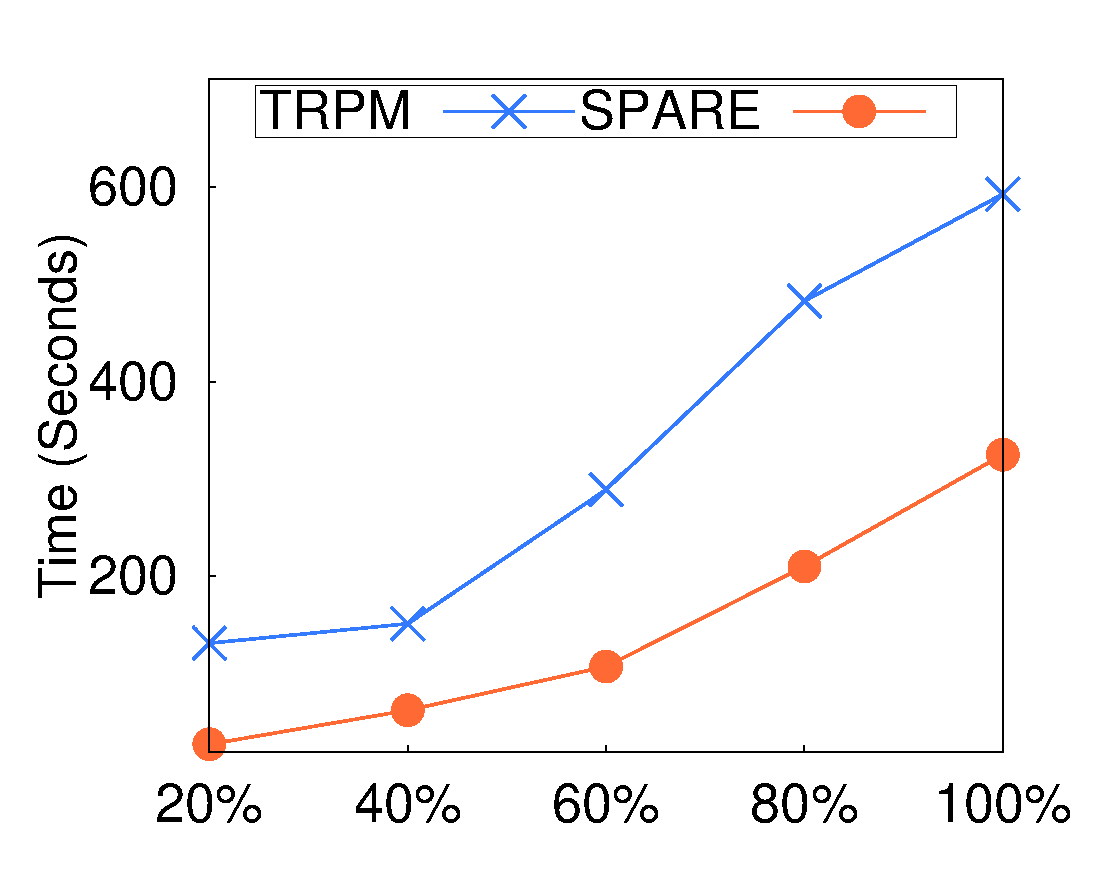
\includegraphics[width=\textwidth]{/exp/performance/shopping_vary_o.eps}
        \caption{Shopping vary $O_r$}
    \end{subfigure}
 	 \begin{subfigure}[b]{0.22\textwidth}
        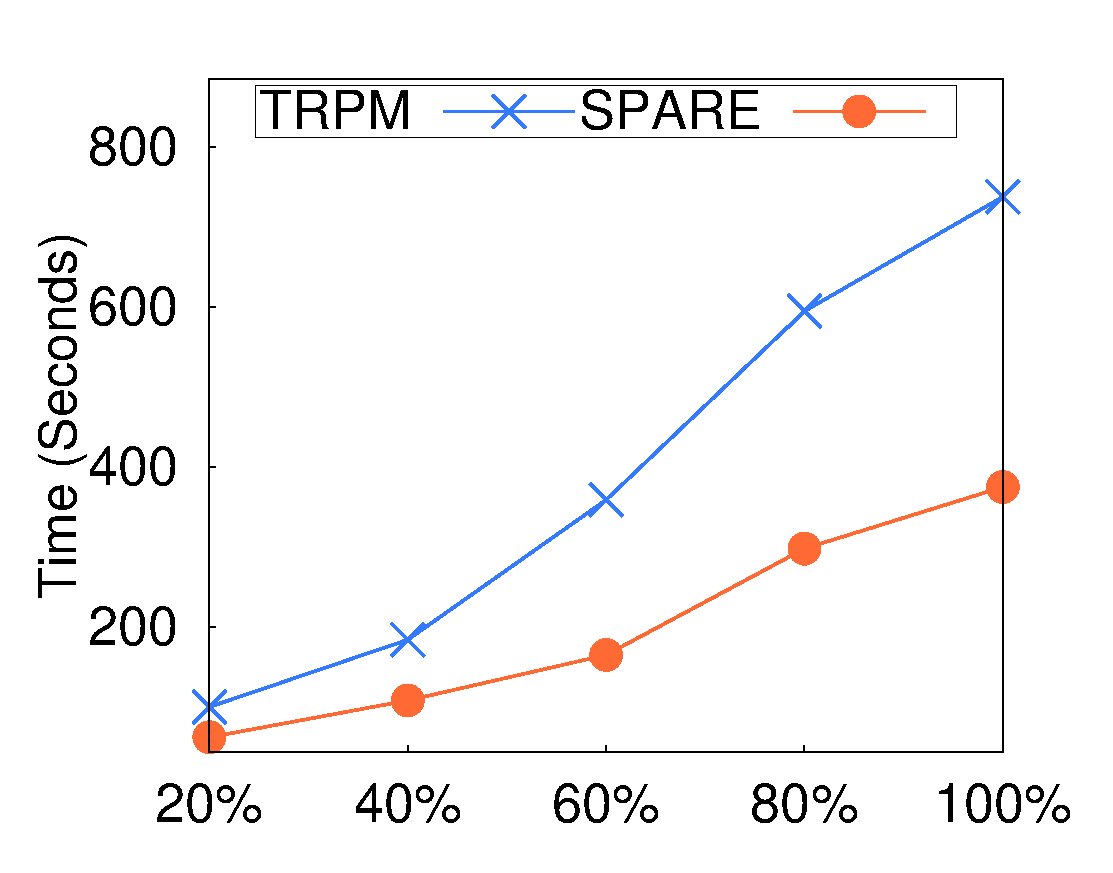
\includegraphics[width=\textwidth]{/exp/performance/geolife_vary_o.eps}
        \caption{Geolife vary $O_r$}
    \end{subfigure}
    	 \begin{subfigure}[b]{0.22\textwidth}
        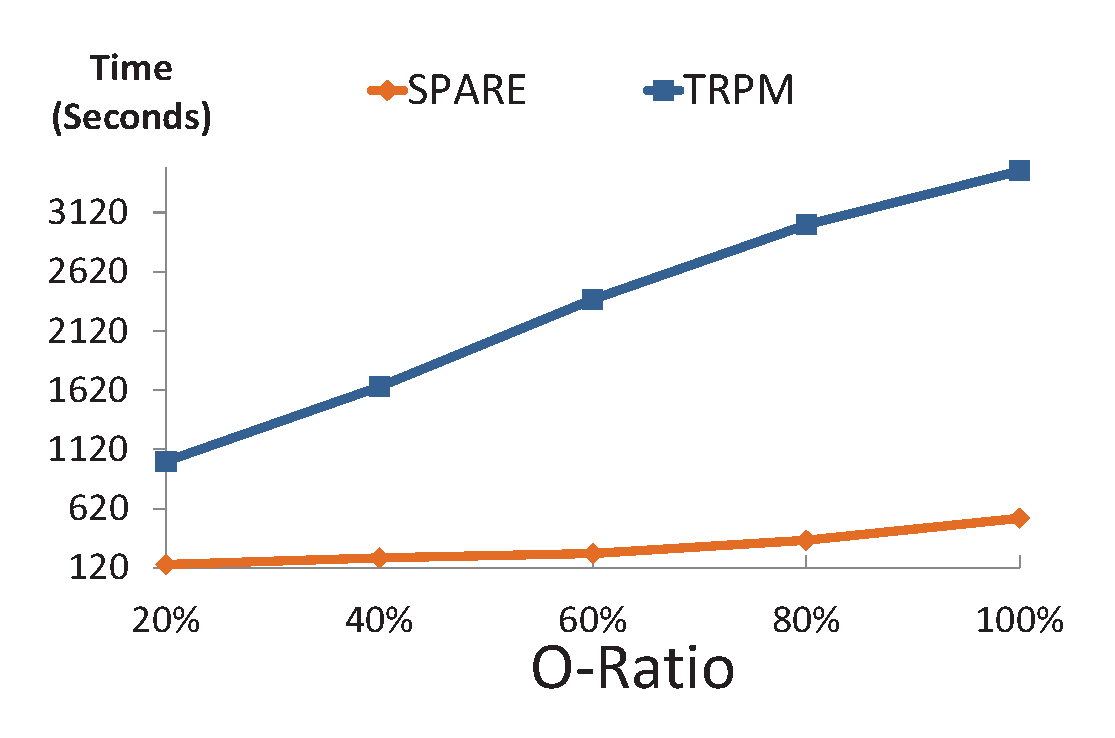
\includegraphics[width=\textwidth]{/exp/performance/taxi_vary_o.eps}
        \caption{Taxi vary $O_r$}
    \end{subfigure}
    \begin{subfigure}[b]{0.22\textwidth}
	 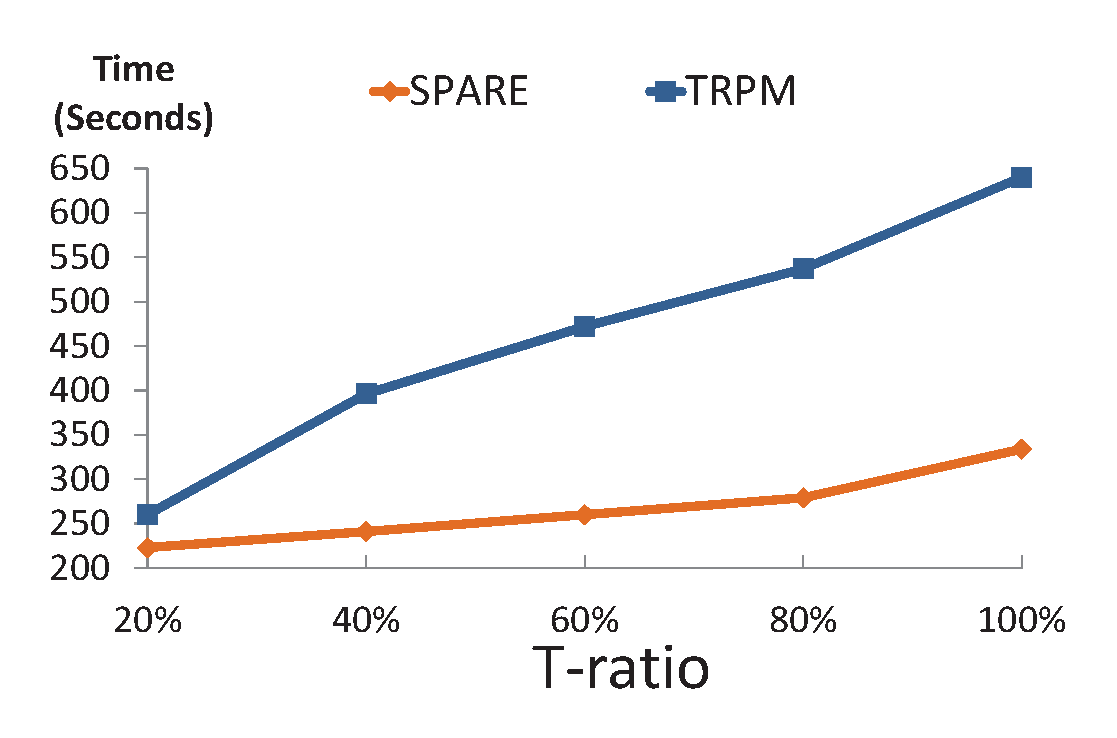
\includegraphics[width=\textwidth]{/exp/performance/shopping_vary_t.eps}
        \caption{Shopping vary $T_r$}
    \end{subfigure}
 	 \begin{subfigure}[b]{0.22\textwidth}
        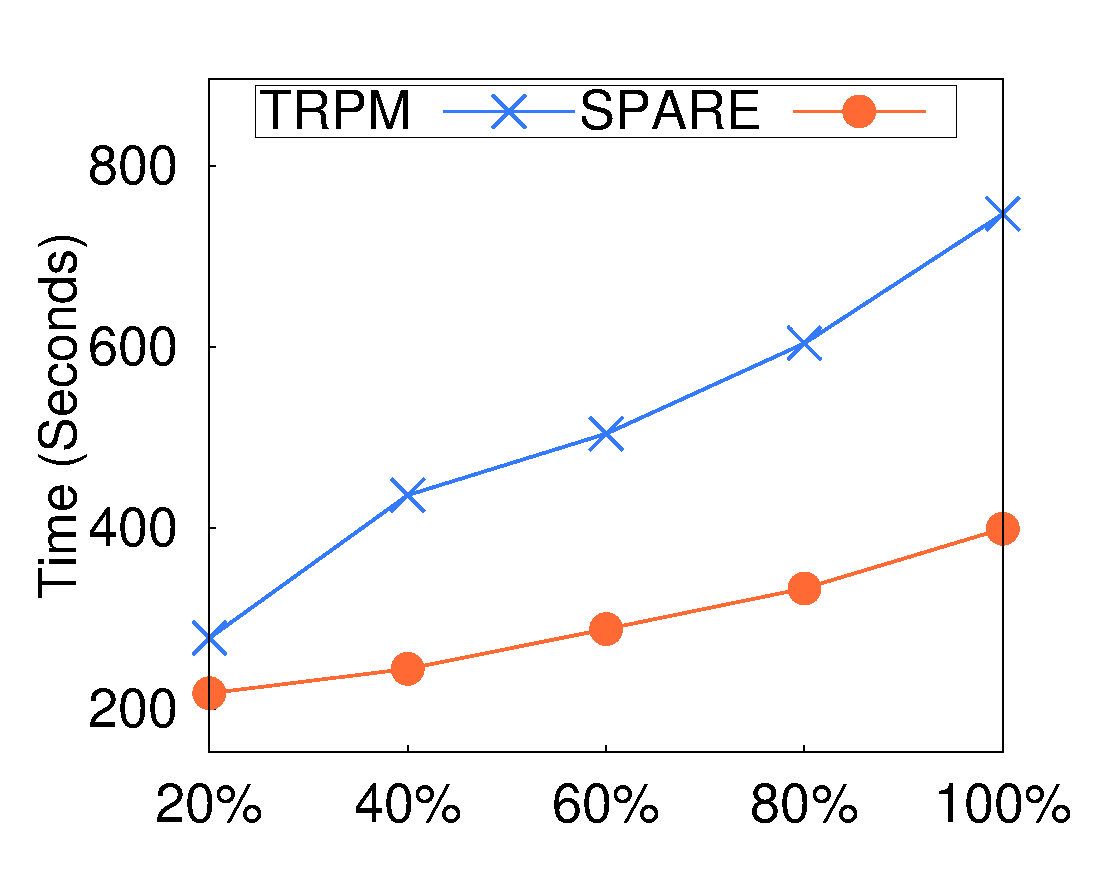
\includegraphics[width=\textwidth]{/exp/performance/geolife_vary_t.eps}
        \caption{Geolife vary $T_r$}
    \end{subfigure}
    	 \begin{subfigure}[b]{0.22\textwidth}
        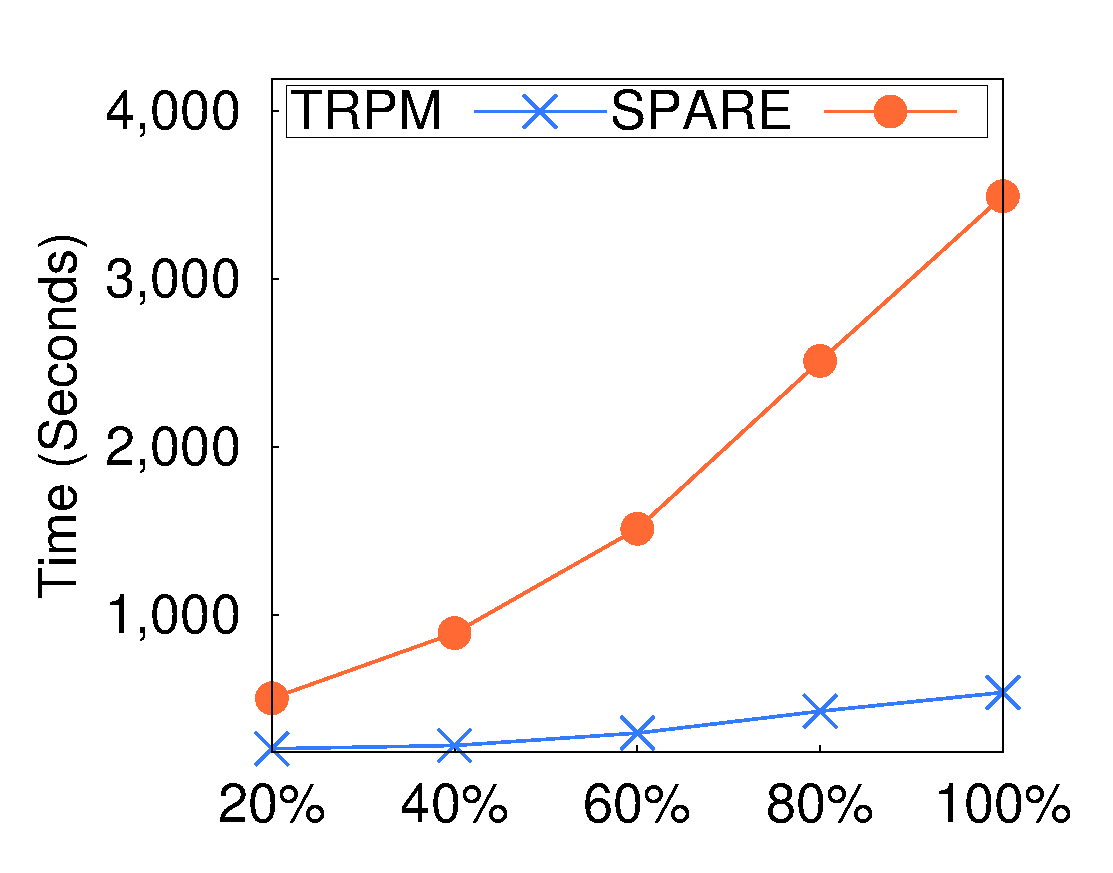
\includegraphics[width=\textwidth]{/exp/performance/taxi_vary_t.eps}
        \caption{Taxi vary $T_r$}
    \end{subfigure}
 \caption{Scalability of SPARE and TRPM wrt. $O_r$ and $T_r$}
 \label{exp:performance_vary_OT}
\end{figure}



\subsection{Analysis of SPARE framework}
In this part, we extensively evaluate the advantage brought by 
sequence simplification and load balancing techniques.

\subsubsection{Power of sequence simplification}
One of the core techniques used in SPARE is the \emph{sequence simplification} (see Section 5.2.1). 
As shown in  Algorithm~\ref{algo:apriori_mining}, we use $\mathtt{sim}(T)$
to prune false candidates. To study the power of sequence simplification,
we collect the following two statistics: (1) the number of pairs that
are shuffled to reducers and (2) the number of pairs that
are fed to the Apirori enumeration. The difference of the two quantities
the the pairs that are pruned by the sequence simplification.
%
%we collect the total number of pairs that are pruned before apriori enumeration.
%In particular, we compare the number of 
%The number of pairs prior to pruning is counted in the load balance stage, while
%the number of pairs after pruning is counted in the Apriori stage.
The
statistics are shown in Table~\ref{tbl:pruning} under default parameters. The result states that the \emph{sequence simplification} is a very powerful pruning technique. It cuts off near 90\% of the initial pairs, which significantly reduces the costs
of later enumerations. This confirms the necessity and usefulness of design such a technique.


\begin{table}[h]
\begin{tabular}{|l|c|c|c|}
\hline 
\textbf{Data Set} & \textbf{Shopping} & \textbf{Geolife} & \textbf{Taxi} \\ 
\hline 
Before pruning & 878,309 &  1,134,228 & 2,210,101 \\ 
\hline 
After pruning & 76,672 & 123,410 & 270,921 \\ 
\hline 
Prune ratio & 91.2\% & 89.1\% & 87.7\% \\ 
\hline 
\end{tabular} 
%
%\begin{tabular}{|c|c|c|c|}
%\hline 
%\textbf{Dataset} & \textbf{Initial Candidates} & \textbf{Real Candidates} & \textbf{Prune-Ratio} \\ 
%\hline 
%Shopping & 878,309 & 76,672 &  91.2\%\\ 
%\hline 
%Geolife & 1,134,228 & 123,410 & 89.1\% \\ 
%\hline 
%Taxi & 2,210,101 & 270.921 & 87.7\% \\ 
%\hline 
%\end{tabular} 
\caption{Pruning power of SPARE}
\label{tbl:pruning}
\end{table}

\begin{figure}[h]
\centering
	\begin{subfigure}[b]{0.22\textwidth}
        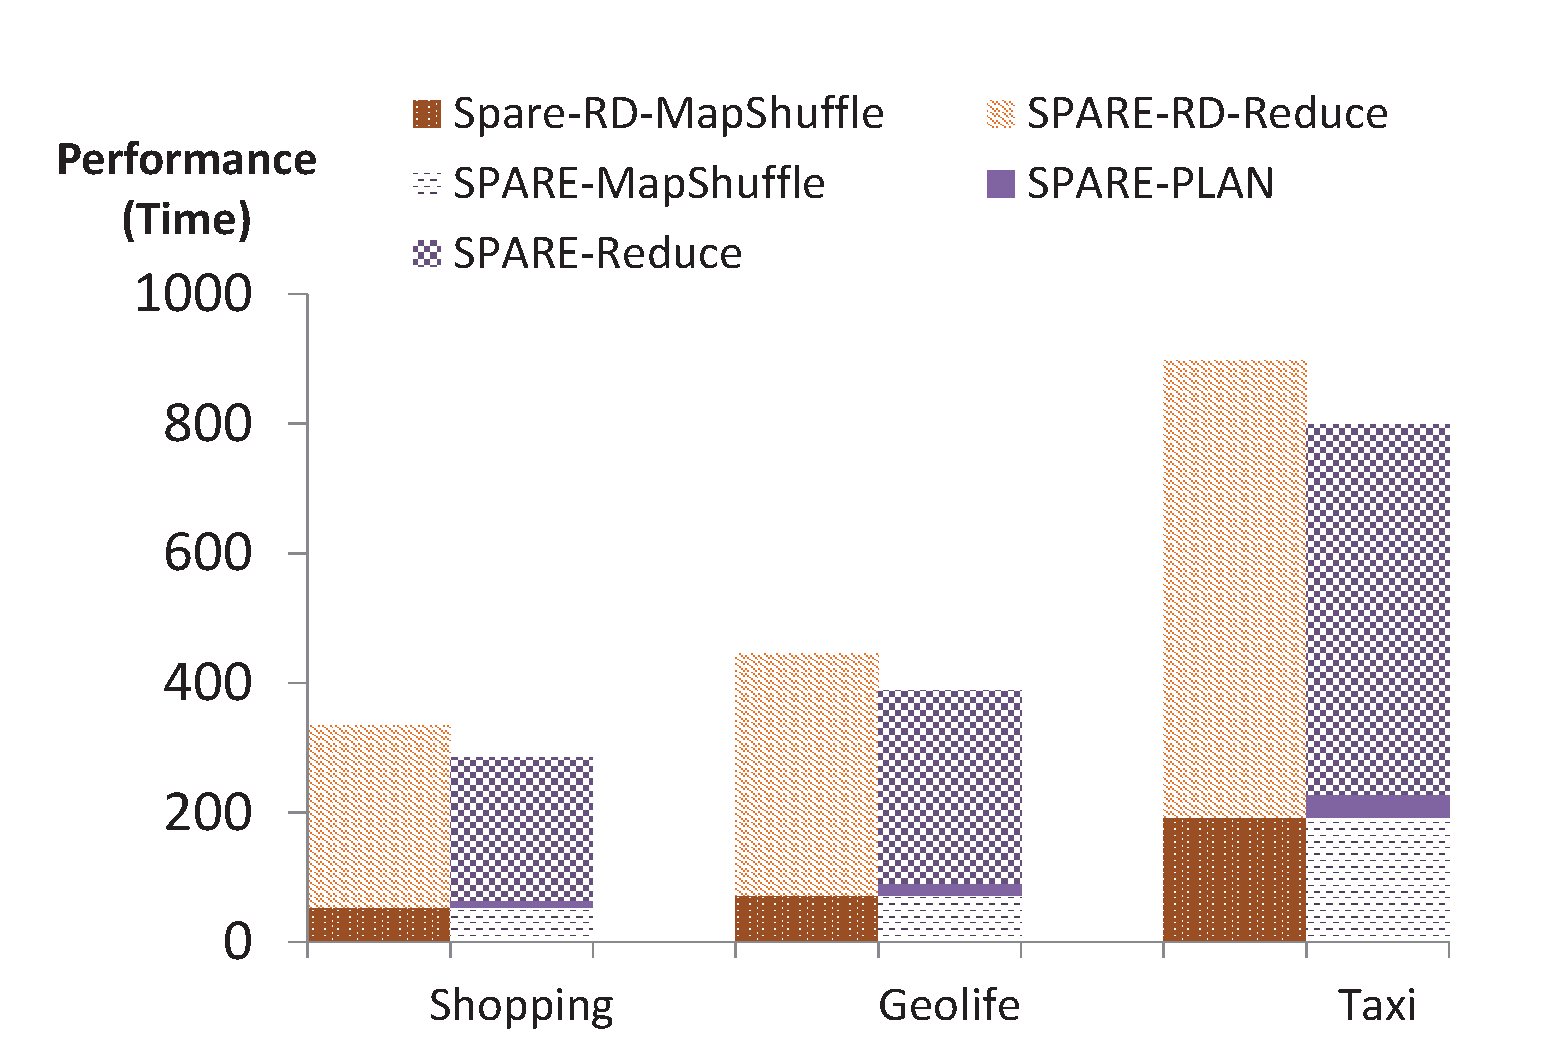
\includegraphics[width=\textwidth]{/exp/spare/detail.eps}
        \caption{Decomposed running time}
    \end{subfigure}
 	 \begin{subfigure}[b]{0.22\textwidth}
        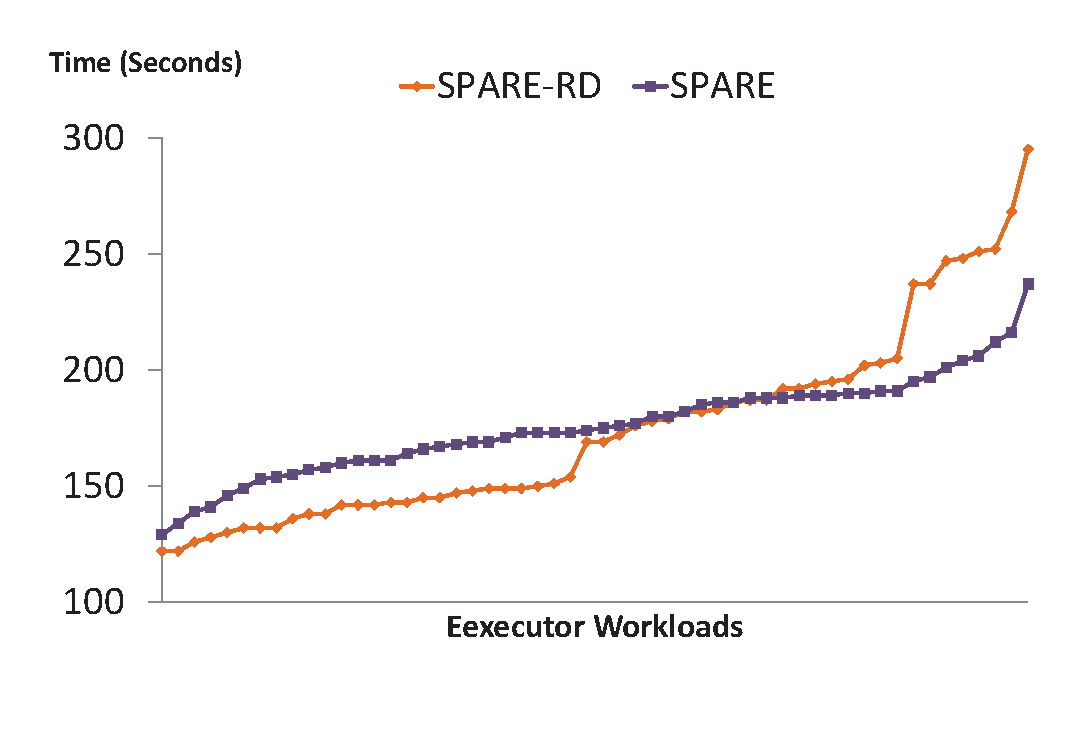
\includegraphics[width=\textwidth]{/exp/spare/wl-shopping.eps}
        \caption{Workload in Shopping}
    \end{subfigure}
    \begin{subfigure}[b]{0.22\textwidth}
        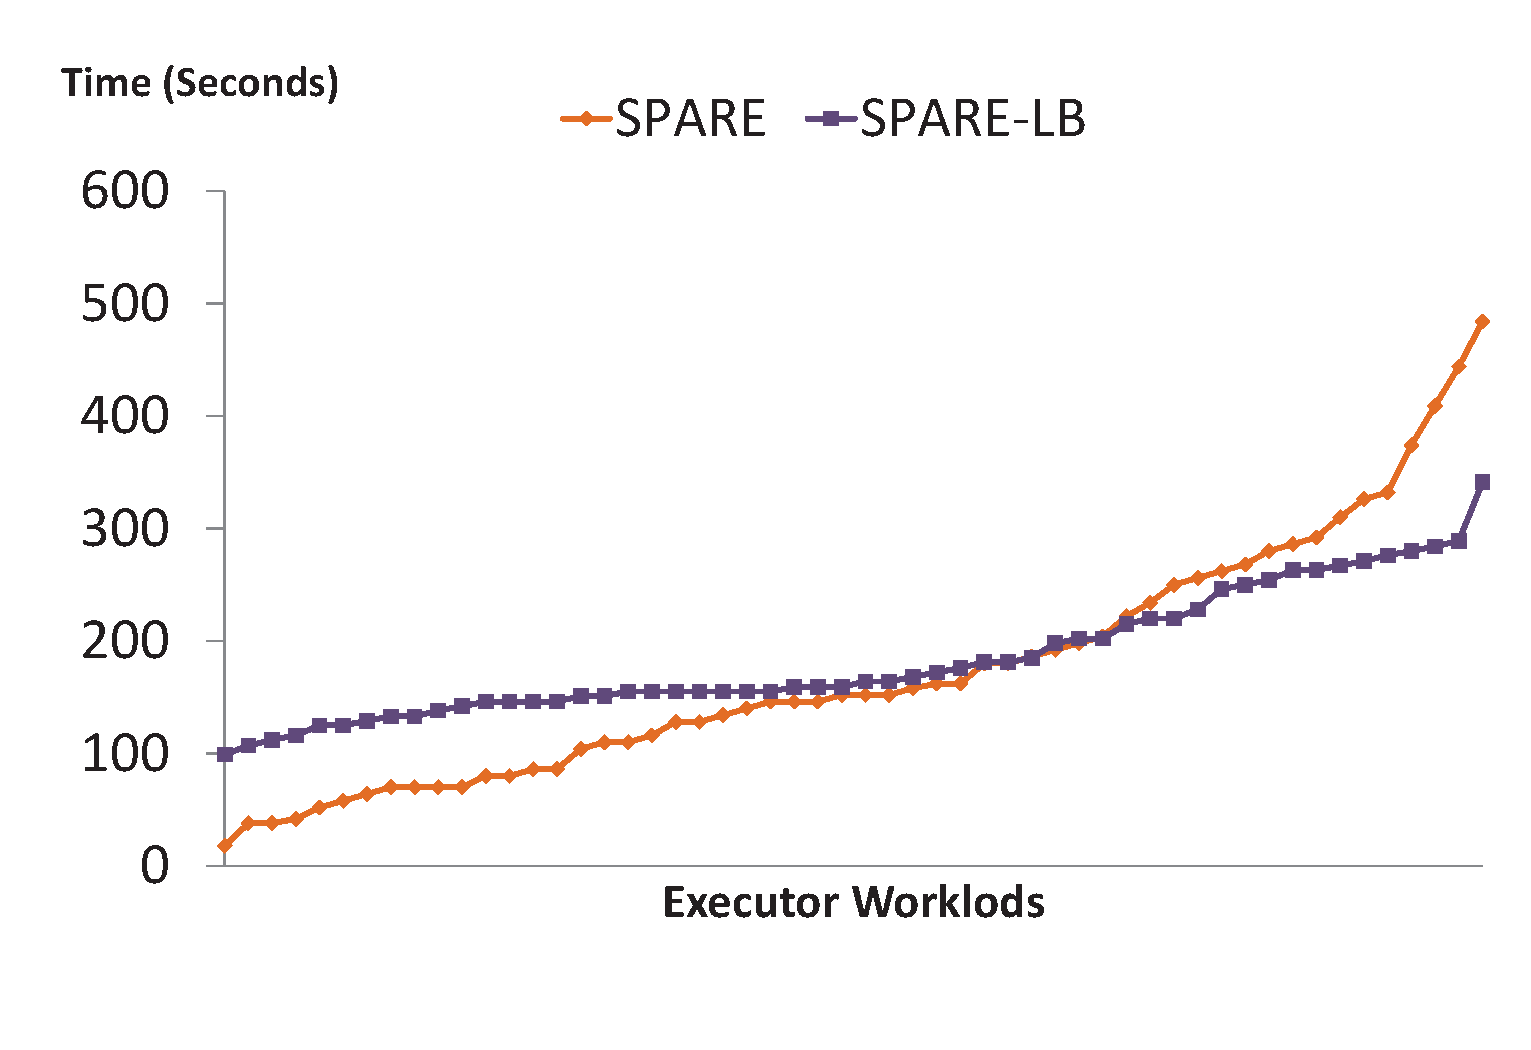
\includegraphics[width=\textwidth]{/exp/spare/wl-geolife.eps}
        \caption{Workload in Geolife}
    \end{subfigure}  
    \begin{subfigure}[b]{0.22\textwidth}
        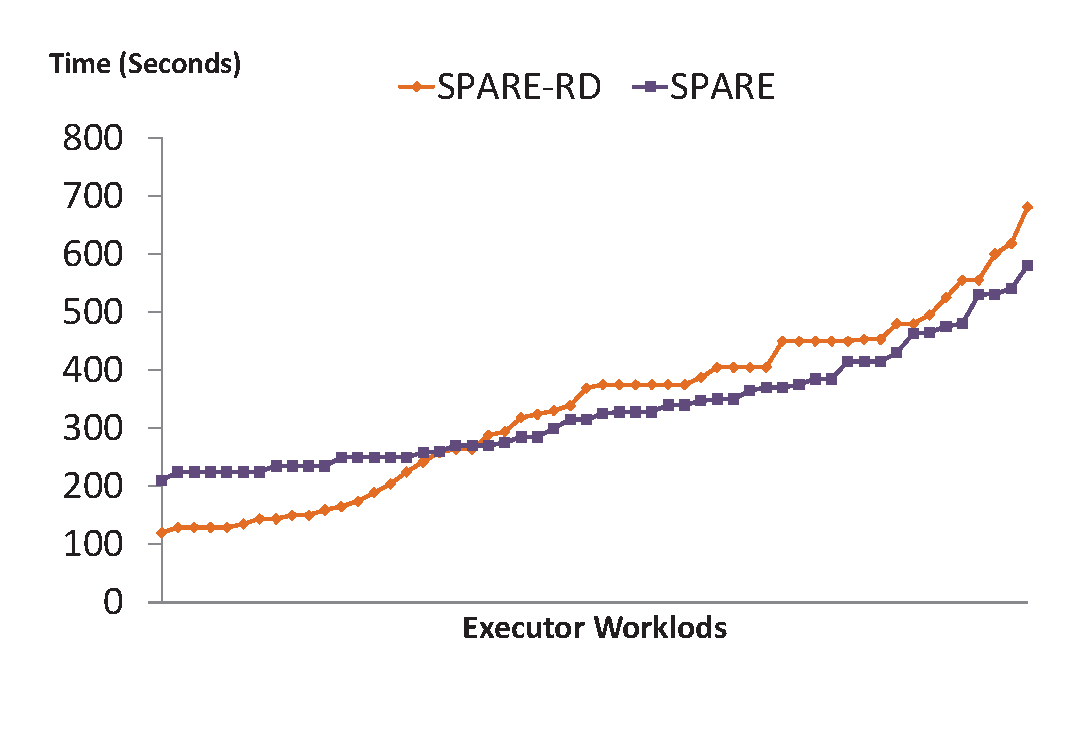
\includegraphics[width=\textwidth]{/exp/spare/wl-taxi.eps}
        \caption{Workload in Taxi}
    \end{subfigure}
\caption{Load balance of SPARE and SPARE-LB}
\label{exp:wl}
\end{figure}

\subsubsection{Load Balance}
To study why SPARE is more efficient,
we analyze the running time of  SPARE
each map-reduce stage.  To compare with, we use
the SPARE-RD which is SPARE with random task allocation as a baseline.
The detail anatomy is shown in Figure~\ref{exp:wl}(a).
We can see that on all three datasets, the reduce phase for both SPARE and SPARE-RD takes the majority time. The overall improvement of SPARE is around 10-13\%
under the default settings. We observe that the map and shuffle time
of SPARE and SPARE-RD are identical, where SPARE spends a very small portion of extra time (4\% of the total time)
in applying the best-fit strategy. The time spent is worthwhile
as in the reduce phase SPARE saves around 20\% of the time. 

We then look at the workload distribution of SPARE and SPARE-RD on real datasets. 
We collect the statistics from executors
and report their reduce times in Figure~\ref{exp:wl}. 
The figures show that SPARE is able to provide a more balanced 
task allocation in all three cases. Since SPARE-RD takes random assignment
of stars, it is likely to assign many large stars to the same executor. 
In general cases, SPARE is recommended as 
it offers more efficiency while takes only a small extra time for planning.


\eat{
\subsubsection{Scalability}
We then study the scalability of SPARE-LB from two aspects. 
First, we fix the computing power and vary the size of dataset.
We perform a random sample from the tree dataset and the results of SPARE-LB are shown in Figures~\ref{fig:scalability-wl}. As the figures show, SPARE-LB grows almost linearly wrt $|O|$ and $|T|$. This suggests a good scalability. 
Note that, as shown in Figure~\ref{fig:related_work_scalability}, a centralized algorithm runs more than a hundred times slower than SPARE for the same scale of data. This confirms the superiority of our parallel

\begin{figure}[h]
\begin{subfigure}[b]{0.22\textwidth}
\centering
    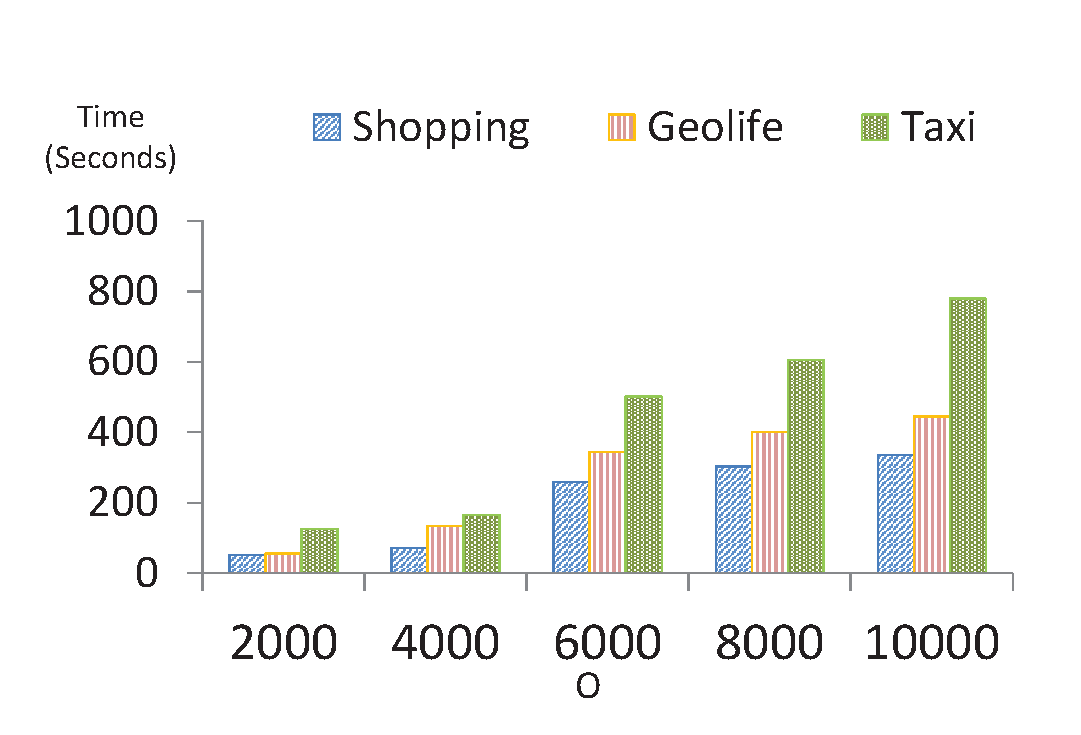
\includegraphics[width=\textwidth]{/exp/spare/scalability-vary-O.eps}
        \caption{Scalability vary $|O|$}
    \end{subfigure}
 	 \begin{subfigure}[b]{0.22\textwidth}
        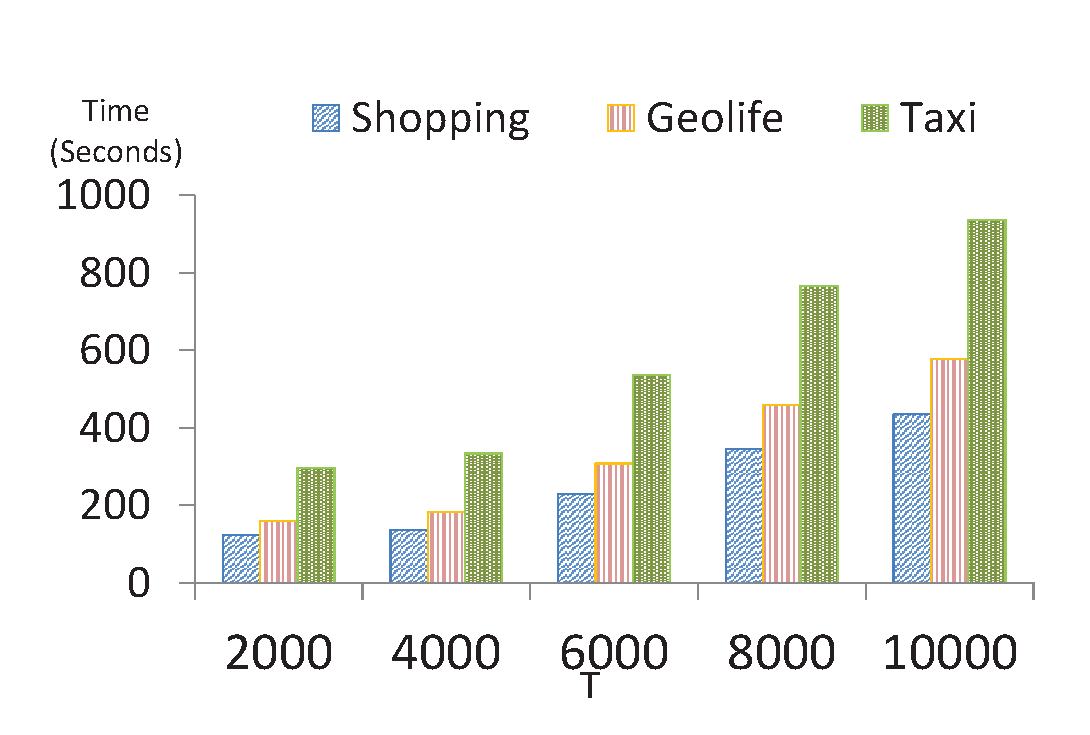
\includegraphics[width=\textwidth]{/exp/spare/scalability-vary-T.eps}
        \caption{Scalability vary $|T|$}
    \end{subfigure}
 \caption{Scalability of SPARE-LB wrt. different data sizes}
 \label{fig:scalability-wl}
\end{figure}

Second, we fix the work load and vary the number of executors.
The result are presented in Figure~\ref{exp:scalability}.
We can see that SPARE achieves good scalability under all three cases. 
For instance, for Taxi dataset, when the executors rises from 10 to 50, 
the performance improves 4.8 times which is almost linear to the increase of executors. Such pattern also holds for the other two datasets. The reason for the good scalablity is that SPARE partitions the trajectories by objects and partitions are perfectly independent. Therefore, when the number of executors $N << |O|$, SPARE can always speed up by adding more executors.
\begin{figure}[h]
\centering
   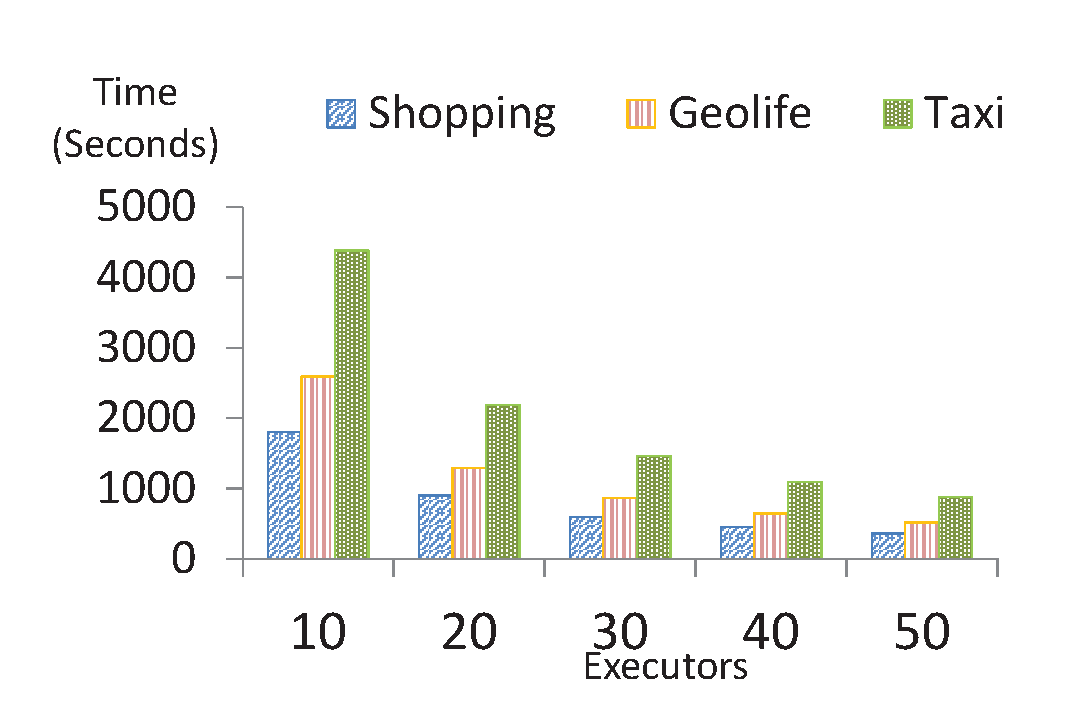
\includegraphics[width=0.3\textwidth]{/exp/spare/scalability.eps}
\caption{Scalability of SPARE-LB vary. $N$.}
\label{exp:scalability}
\end{figure}
}

\subsection{Scalability and Comparison with Existing Solutions}
We then study the scalability of our schemes.
Since existing solutions run on a single machine, it is interesting to compare their
performances. We choose \emph{platoon} as the comparing scheme as it is
generic and more efficient than \emph{swarm} and \emph{group}
The results are presented in Figure~\ref{exp:scalability}. There are two observations.
First, the centralized scheme (e.g. platoon) are not suitable for discover
patterns in large-scale trajectories. It takes near 16 hours for discovering \emph{platoon}s
in Taxi data. As a comparison, our TRPM and SPARE achieves 2.4 times and 7.1 times speedup.
This is because even there is only 1 machine, our TRPM and SPARE is still able to leverage
the 15 cores in the machine for parallelism. Second, we see that both TRPM and SPARE
demonstrate good scalability wrt. $N$. As the number of machines increases from 1 to 11 (i.e., 11 times),
both TRPM and SPARE achieves near 11 times speedup. Note that SPARE at most achieves 94 times
speedup as compared to \emph{platoon} using all 11 machines.

\begin{figure*}[t]
\centering
\begin{subfigure}[b]{0.32\textwidth}
    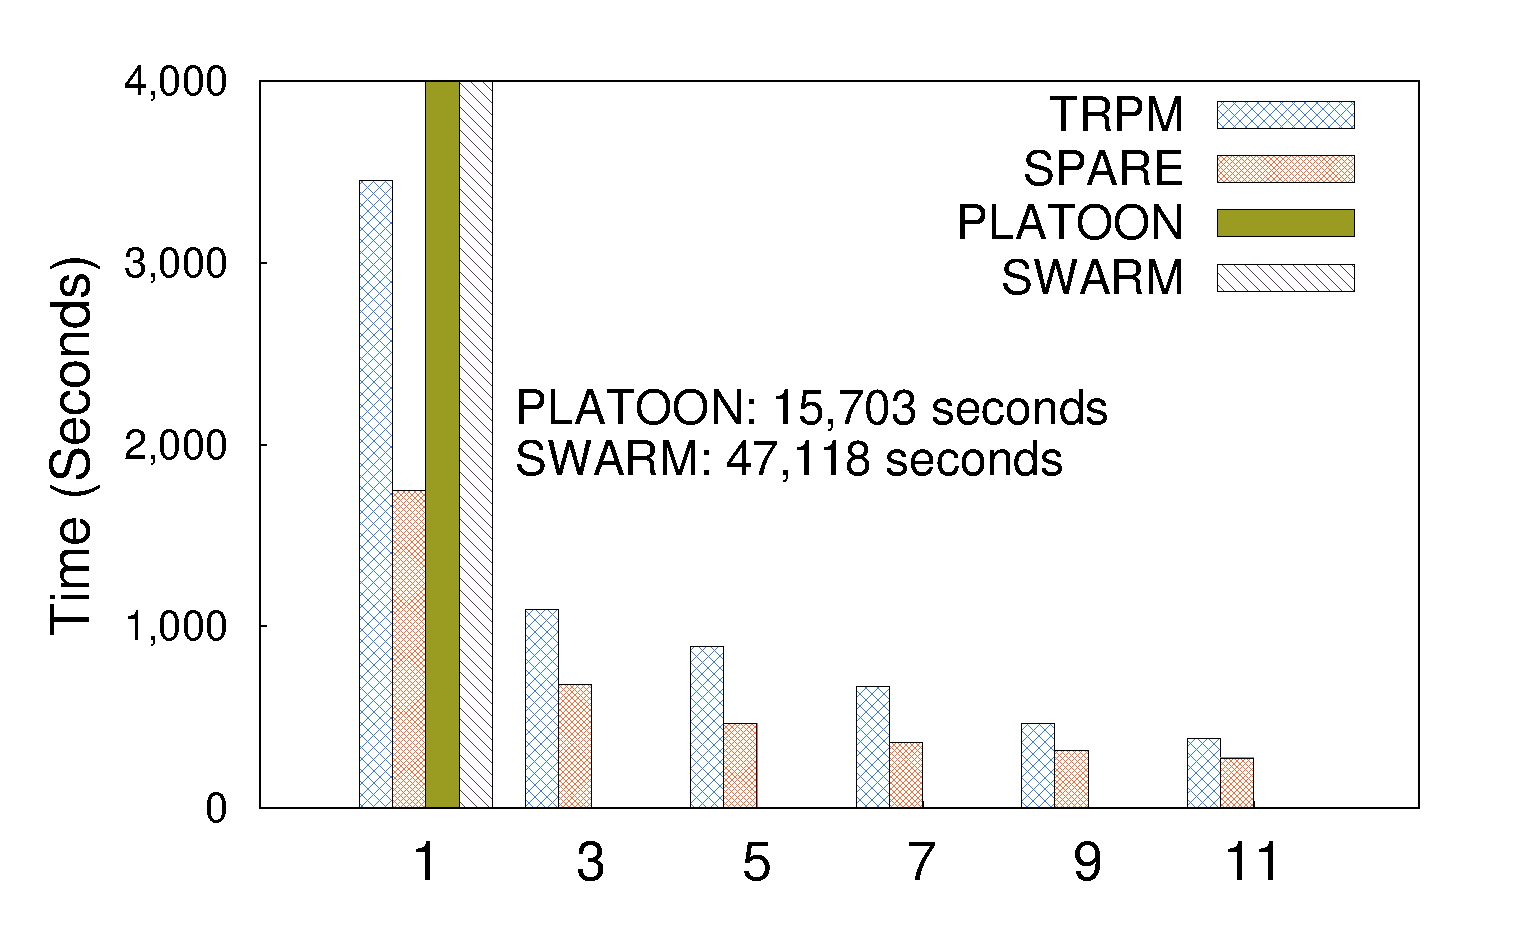
\includegraphics[width=\textwidth]{/exp/spare/scalability-shopping.eps}
        \caption{Shopping vary $N$}
    \end{subfigure}
 	 \begin{subfigure}[b]{0.32\textwidth}
        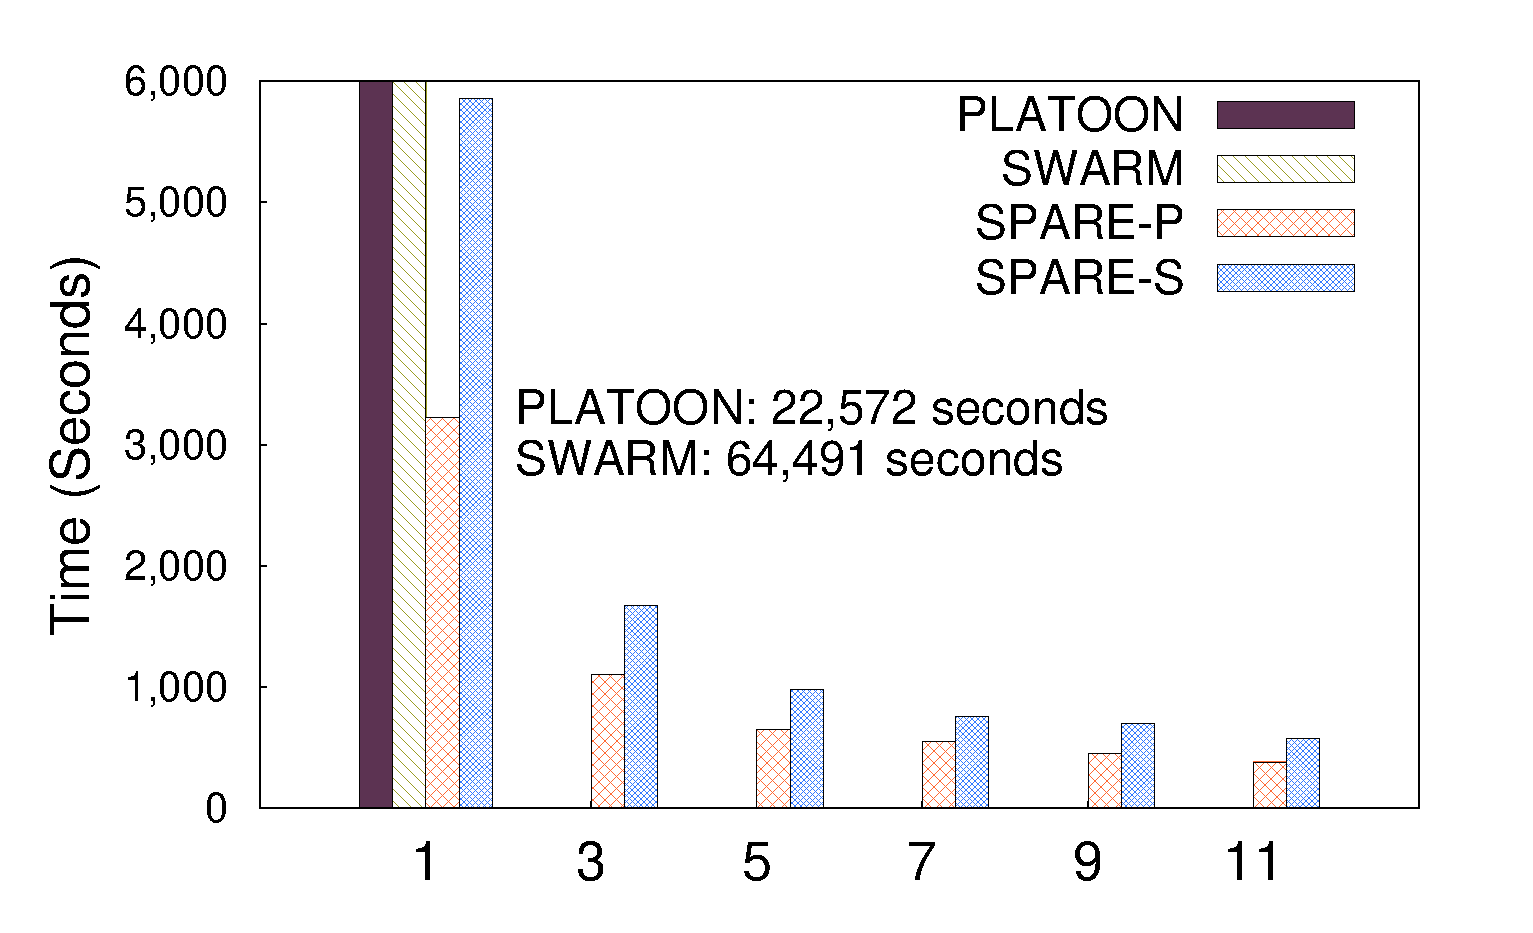
\includegraphics[width=\textwidth]{/exp/spare/scalability-geolife.eps}
        \caption{Geolife vary $N$}
    \end{subfigure}
    	 \begin{subfigure}[b]{0.32\textwidth}
        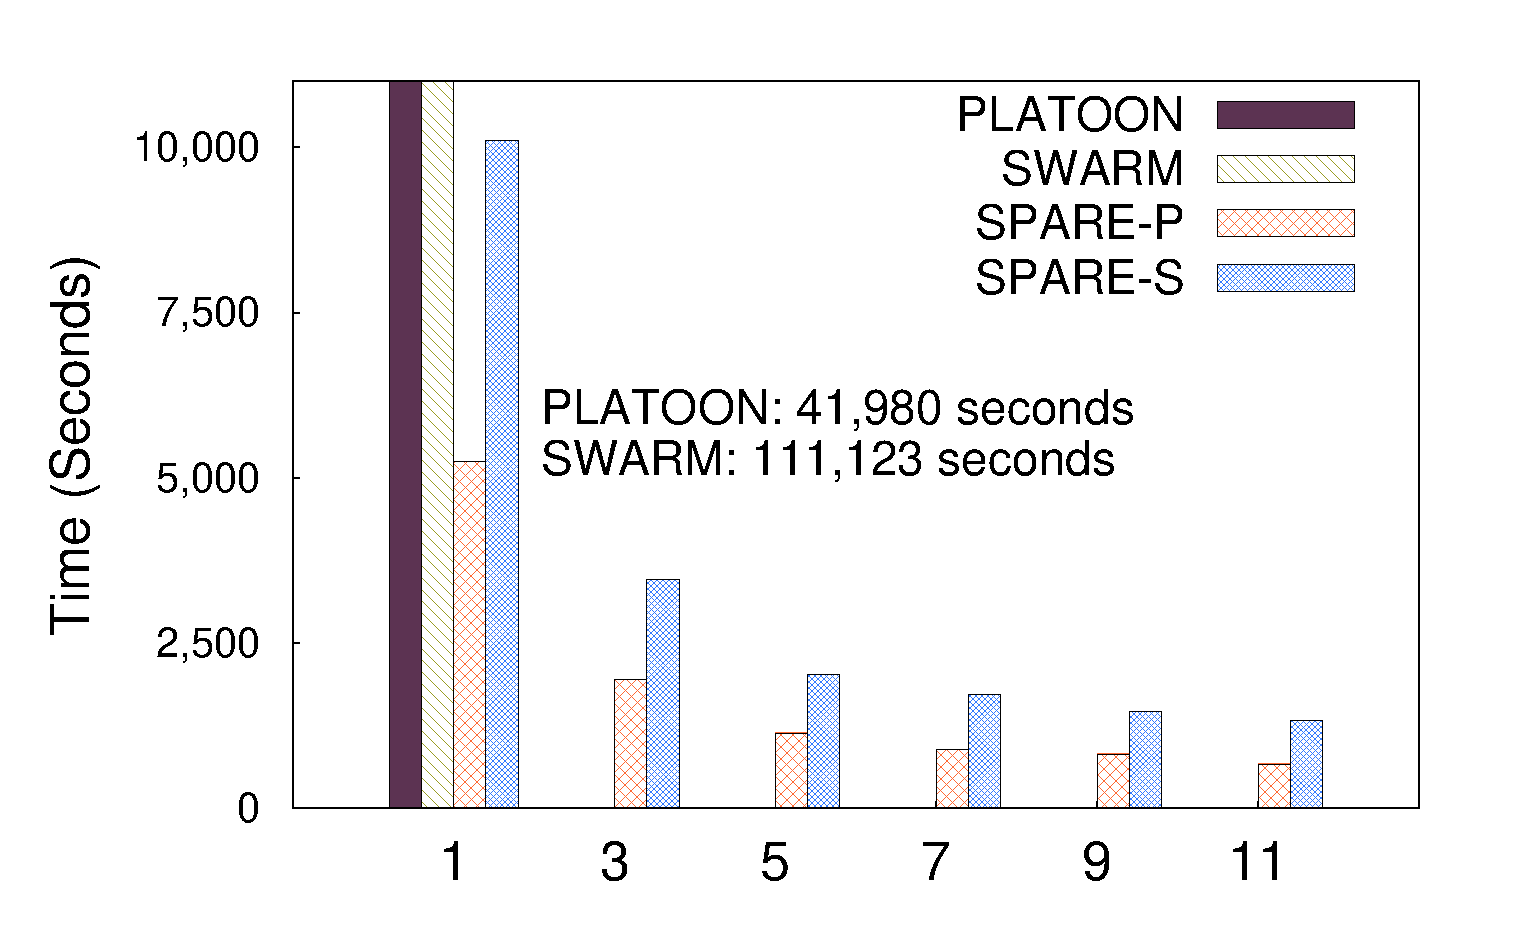
\includegraphics[width=\textwidth]{/exp/spare/scalability-taxi.eps}
        \caption{Taxi vary $N$}
    \end{subfigure}
 \caption{Scalability of SPARE and TRPM wrt. $N$}
 \label{exp:scalability}
\end{figure*}